\newcommand{\EF}{$\mathcal{E.F.}$ }
\newcommand{\pmf}{\textit{pmf} }
\newcommand{\suffstat}{\textit{sufficient statistics} }
\newcommand{\canonparam}{\textit{canonical parameters} }
\newcommand{\cumfun}{\textit{cumulant function} }
\newcommand{\natparam}{\textit{natural parameters} }

\subsection{Exponential Family}

The Exponential Family (\EF) is a parametric family of probability distribution. Many of the common distribution are part of the \EF. Here are some examples: 
\begin{itemize}
	\item Bernulli Distribution.
	\item Normal Distribution.
	\item Categorical Distribution.
	\item Multinomial Distribution.
	\item Poisson Distribution.
\end{itemize}
\EF represents a convienient framework to represent many distributions at the same time. A distribution belongs to the \EF if its Probability Mass Function (\pmf) $p(x|\theta)$ can be written in the following form:
\begin{equation}
	p(x|\theta) = h(x)\exp(\eta(\theta)^T\phi(x)+A(\eta(\theta)))
	\label{eq:EF}
\end{equation}
Each of these terms has its own meaning. Firstly, $phi(x)$ is known as the \suffstat (why? we will discuss this later). Secondly, $\eta(\theta)$ is called the \canonparam while $\theta$ is called \natparam. Thirdly, $A(\eta(\theta))$ is known as \cumfun and it has the following form:

\begin{equation}
	A(\eta(\theta)) = \log \int h(x)exp(\eta(\theta)^T\phi(x))dx
\end{equation}

$A(\eta(\theta))$ is nothing more than the logarithm of the normalization factor of the distribution. That is, the term that makes sure that the integral sums up to $1$.

Where $\theta$ represents the parameters. Let's see some examples starting with the Bernulli Distribution ($Ber(x|\theta)$ with $x\in{1,-1}$). Usually, the Bernulli Distribution is written as follows:

\begin{equation}
	Ber(x|\theta) = \theta^x(1-\theta)^{1-x}
	\label{eq:bernulli}
\end{equation}

In Figure~\ref{fig:bernulli-plot}, You have a plot for $Ber(x|\theta=0.3)$.
Now, we can proceeds by writing the the distribution in \ref{eq:bernulli} in the \EF form (\ref{eq:EF}). 
\begin{figure}
	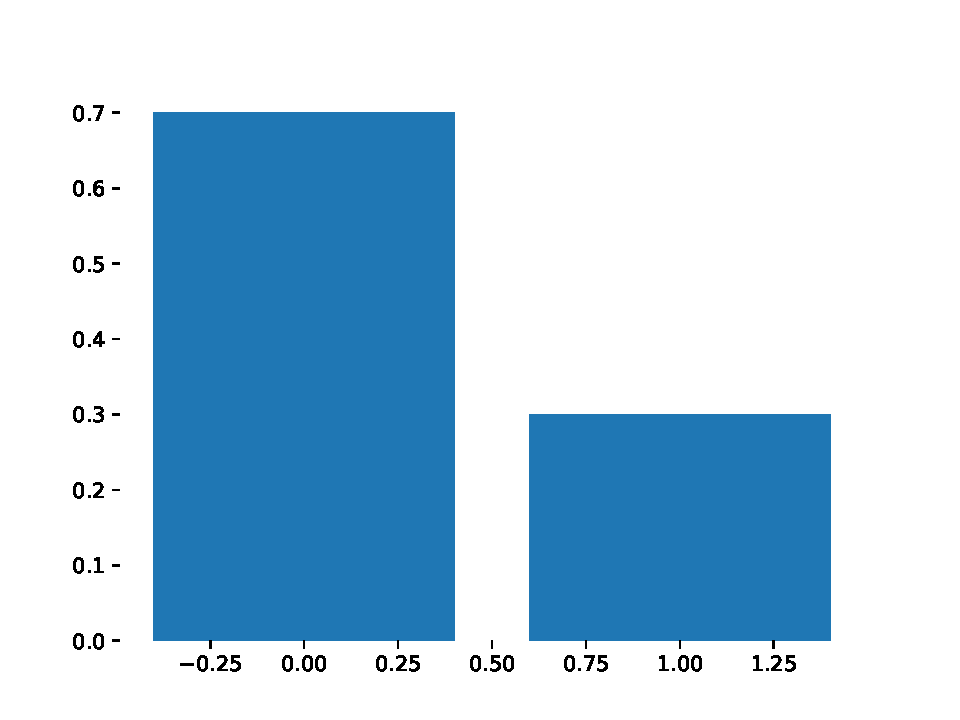
\includegraphics[width=7cm]{GeneralizedLinearModels/figs/bernulli.pdf}	
	\caption{Bernulli distribution examples with $\theta=.3$}
	\label{fig:bernulli-plot}
\end{figure}

\begin{align}
	Ber(x|\theta) = \theta^x(1-\theta)^{1-x} = \\
	\exp(\log(\theta^x(1-\theta)^{1-x})) = \\
	\exp(x\log(\theta)+(1-x)log(1-\theta)) = \\
	\exp(\eta(\theta)\phi(x)+A(\eta(\theta)))
	\label{th:bref}
\end{align}

Where:

\begin{align}
	\eta(\theta) =
	\begin{bmatrix}
		\log(\theta)\\
		\log(1-\theta)
	\end{bmatrix},
	\phi(x) = 
	\begin{bmatrix}
		x\\
		1-x
	\end{bmatrix},
	A(\eta(\theta)) = 0
\end{align}

